\newcommand{\ttt}[1]{\texttt{#1}}
\newcommand{\icc}{\texttt{icc}}
\newcommand{\gcc}{\texttt{gcc}}

\subsection{Compiler Flags and Annotations}
Compilers such as \icc{} and \gcc{} are equipped with a wide variety of command
line flags that can be used to increase the performance of the compiled code.
Similarly, the compilers understand a set of source code annotations that can
inform the compiler of certain assumptions it can make to optimize code.
Empirically, we found that that \icc{} produced the fastest code; in this
section, we present the \icc{} flags and annotations we explored.

\subsubsection{Compiler Flags}
\begin{itemize}
  \item \ttt{-xCORE-AVX2}:
    The \ttt{-x} flag informs the compiler which platform-specific
    optimizations it can use. Since we have a Xeon E5 v3 processor, we use the
    \ttt{CORE-AVX2} flag.

  \item \ttt{-fast}:
    The \ttt{-fast} flag enables entire program optimization. Its a meta-flag
    enables a set of other flags that increase performance including \ttt{-O3},
    \ttt{-ipo}, and \ttt{no-prec-div}.

  \item \ttt{-ansi-alias}:
    The \ttt{-ansi-alias} flag tells the compiler that our code adheres to the
    ANSI alias guidelines and allows the compiler to make aggressive
    optimizations.

  \item \ttt{-no-prec-div}:
    The \ttt{-no-prec-div} flag decreases the accuracy of floating point
    division at the benefit of increased performance. This is also enabled by
    \ttt{-fast}.

  \item \ttt{-ipo}:
    The \ttt{-ipo} flag informs the compiler to perform inter-process
    optimization. When \ttt{-ipo} is enabled, the compiler will optimize code
    from multiple files when they are linked together.

  \item \ttt{-prof-gen} and \ttt{-prof-use}:
    The \ttt{-prof-gen} and \ttt{-prof-use} allow for profile-guided
    optimization. A binary compiled with \ttt{-prof-gen} is instrumented such
    that whenever it runs, it generates a profile documenting the most
    frequently executed code paths. A binary compiled with \ttt{-prof-use} is
    built to optimize the frequently executed code paths documented in the
    profiles.
\end{itemize}

% TODO: explain what worked

\subsubsection{Compiler Annotations}
% TODO: align and restrict
% TODO: explain what worked

\begin{figure}[h]
  \centering
  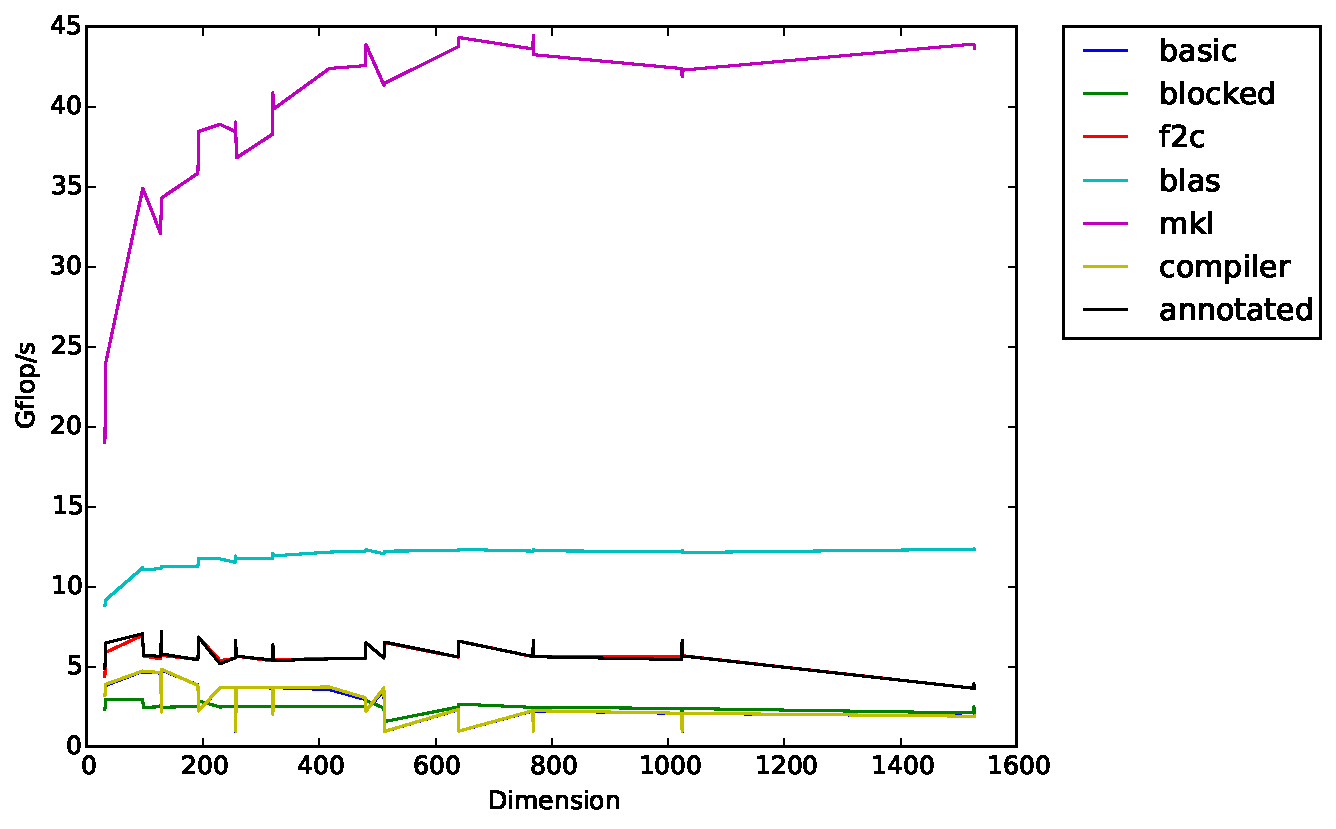
\includegraphics[width=\textwidth]{timing_compiler.pdf}
  \caption{Performance of compiler flags and annotations.}
  \label{fig:compiler}
\end{figure}
